\chapter{Параллельные прямые и плоскости}\label{ch:ch3}

\begingroup
\setlength{\intextsep}{10pt plus 2pt minus 2pt}
\setlength{\textfloatsep}{12pt plus 2pt minus 2pt}

% А. П. Киселёв, «Элементарная геометрия», 23-е издание, 1914. Печатные с. 283–292.
% Страницы скана планиметрии на 11 больше печатных.
\newcommand*{\kiselevPlanimetryPage}[2]{%
    \href{https://commons.wikimedia.org/wiki/File:\%D0\%90._\%D0\%9F._\%D0\%9A\%D0\%B8\%D1\%81\%D0\%B5\%D0\%BB\%D1\%91\%D0\%B2._\%D0\%AD\%D0\%BB\%D0\%B5\%D0\%BC\%D0\%B5\%D0\%BD\%D1\%82\%D0\%B0\%D1\%80\%D0\%BD\%D0\%B0\%D1\%8F_\%D0\%B3\%D0\%B5\%D0\%BE\%D0\%BC\%D0\%B5\%D1\%82\%D1\%80\%D0\%B8\%D1\%8F_(1914).djvu?page=#1}{#2}%
}

\section*{Параллельные прямые}
\addcontentsline{toc}{section}{Параллельные прямые}

% Печатная с. 283.
\kiselevparagraph{para:skew-and-parallel-lines} \textbf{Предварительное замечание.} Две прямые могут быть расположены в пространстве так, что через них нельзя провести плоскость. Возьмём, например, две такие прямые \(AB\) и \(DE\) (рис.~\ref{fig:kiselev-stereo-314}), из которых одна пересекает некоторую плоскость \(P\), а другая лежит в ней, но не проходит через точку пересечения \(C\). Через такие две прямые нельзя провести плоскость, потому что в противном случае через прямую \(DE\) и точку \(C\) проходили бы две различные плоскости: одна --- \(P\), пересекающая прямую \(AB\), и другая, содержащая её. Это невозможно (\hyperref[item:plane-through-line-and-point]{см.~§~\ref*{para:plane-uniqueness-corollaries}, пункт~\ref*{item:plane-through-line-and-point}}).

\begin{figure}[htbp]
    \centering
    \renewcommand{\thefigure}{314}
    \captionsetup{name=Рис.,labelsep=period}
    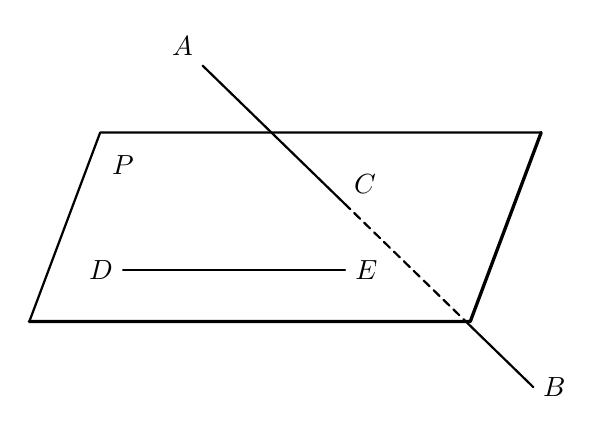
\begin{tikzpicture}[line cap=round,line join=round]
    \coordinate (A) at (-0.95,2);
    \coordinate (C) at (0.85,0.25);
    \coordinate (B) at (3.25,-2.083);
    \path (C) -- (B) coordinate[pos=0.643] (front);
    \draw[thick] (-3.15,-1.25) -- (-2.25,1.15) -- (3.35,1.15);
    \draw[very thick] (-3.15,-1.25) -- (2.45,-1.25) -- (3.35,1.15);
    \draw[thick] (A) -- (C) (front) -- (B);
    \draw[thick,densely dashed] (C) -- (front);
    \draw[thick] (-1.96,-0.6) node[left] {\(D\)} -- (0.86,-0.6) node[right] {\(E\)};
    \node[above left] at (A) {\(A\)};
    \node[right] at (B) {\(B\)};
    \node[above right] at (C) {\(C\)};
    \node at (-1.96,0.74) {\(P\)};
\end{tikzpicture}

    \caption{Прямые \(AB\) и \(DE\), через которые нельзя провести плоскость}\label{fig:kiselev-stereo-314}
\end{figure}

Две прямые, не лежащие в одной плоскости, конечно, не пересекаются, сколько бы их ни продолжали. Однако их не называют параллельными. Это название оставляют только для тех прямых, которые, \emph{находясь в одной плоскости}, не пересекаются, сколько бы их ни продолжали.

Две прямые, не лежащие в одной плоскости, называются \emph{скрещивающимися}.

В планиметрии мы видели (см.~Планиметрия, \kiselevPlanimetryPage{70}{§~77} и \kiselevPlanimetryPage{71}{§~79}), что через любую точку \emph{плоскости} можно провести прямую, параллельную данной прямой, и притом только одну. То же самое можно сказать о любой точке \emph{пространства}, потому что через точку и данную прямую можно провести плоскость, и только одну.

% Печатная с. 284.
\kiselevparagraph{para:plane-intersects-parallel-lines} \textbf{Теорема. Если плоскость} \(P\) (рис.~\ref{fig:kiselev-stereo-315}) \textbf{пересекает одну из параллельных прямых} \(AB\)\textbf{, то она пересекает и другую} \(CD\)\textbf{.}

\begin{figure}[htbp]
    \centering
    \renewcommand{\thefigure}{315}
    \captionsetup{name=Рис.,labelsep=period}
    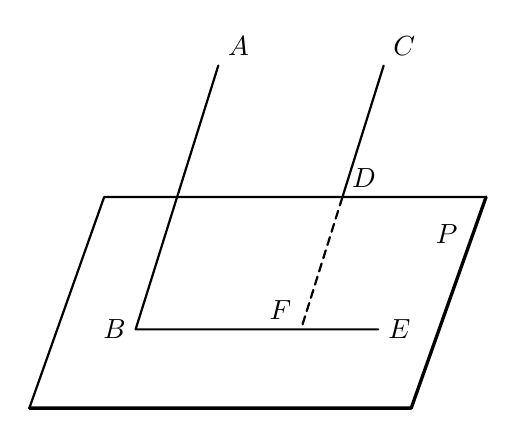
\begin{tikzpicture}[line cap=round,line join=round]
    \coordinate (A) at (-0.5,2.9);
    \coordinate (B) at (-1.55,-0.45);
    \coordinate (C) at (1.6,2.9);
    \coordinate (F) at (0.55,-0.45);
    \path (F) -- (C) coordinate[pos=0.5] (D);
    \draw[thick] (-2.9,-1.45) -- (-1.95,1.23) -- (2.9,1.23);
    \draw[very thick] (-2.9,-1.45) -- (1.95,-1.45) -- (2.9,1.23);
    \draw[thick] (A) -- (B) -- (1.53,-0.45) node[right] {\(E\)};
    \draw[thick] (C) -- (D);
    \draw[thick,densely dashed] (D) -- (F);
    \node[above right] at (A) {\(A\)};
    \node[left] at (B) {\(B\)};
    \node[above right] at (C) {\(C\)};
    \node[above right] at (D) {\(D\)};
    \node[above left] at (F) {\(F\)};
    \node at (2.4,0.76) {\(P\)};
\end{tikzpicture}

    \caption{Плоскость \(P\) пересекает параллельные прямые \(AB\) и \(CD\)}\label{fig:kiselev-stereo-315}
\end{figure}

Проведём через \(AB\) и \(CD\) плоскость. Эта плоскость содержит точку \(B\), в которой прямая \(AB\) пересекается с \(P\). Значит, эта плоскость пересекается с \(P\) по некоторой прямой \(BE\) (\hyperref[para:intersecting-planes]{см.~§~\ref*{para:intersecting-planes}}). Эта прямая, находясь в одной плоскости с \(AB\) и \(CD\) и пересекая одну из этих параллельных, должна пересечь и другую (\kiselevPlanimetryPage{71}{см.~Планиметрия, §~80}) в некоторой точке \(F\). Точка \(F\), находясь одновременно на прямой \(BE\) и на прямой \(CD\), должна быть точкой пересечения плоскости \(P\) с прямой \(CD\).

\kiselevparagraph{para:plane-perpendicular-to-parallel-lines} \textbf{Теорема. Если плоскость} \(P\) (рис.~\ref{fig:kiselev-stereo-316}) \textbf{перпендикулярна к одной из параллельных прямых} \(AB\)\textbf{, то она перпендикулярна и к~другой}~\(CD\)\textbf{.}

\begin{figure}[htbp]
    \centering
    \renewcommand{\thefigure}{316}
    \captionsetup{name=Рис.,labelsep=period}
    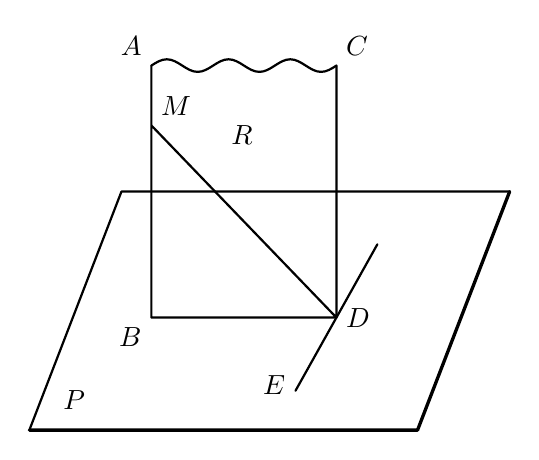
\begin{tikzpicture}[line cap=round,line join=round]
    \coordinate (A) at (-1.4,3);
    \coordinate (B) at (-1.4,-0.2);
    \coordinate (C) at (0.95,3);
    \coordinate (D) at (0.95,-0.2);
    \coordinate (M) at (-1.4,2.24);
    \draw[thick] (-2.95,-1.63) -- (-1.78,1.4) -- (3.15,1.4);
    \draw[very thick] (-2.95,-1.63) -- (1.98,-1.63) -- (3.15,1.4);
    \draw[thick] (A) -- (B) -- (D) -- (C) (M) -- (D);
    % Верхний край плоскости R на рисунке Киселёва показан линией обрыва.
    \draw[thick] (A) sin (-1.204,3.08) cos (-1.008,3)
        sin (-0.812,2.92) cos (-0.616,3)
        sin (-0.42,3.08) cos (-0.224,3)
        sin (-0.028,2.92) cos (0.168,3)
        sin (0.364,3.08) cos (0.56,3)
        sin (0.755,2.92) cos (C);
    \draw[thick] (0.43,-1.13) node[left,yshift=2pt] {\(E\)} -- (D) -- (1.47,0.73);
    \node[above left] at (A) {\(A\)};
    \node[below left] at (B) {\(B\)};
    \node[above right] at (C) {\(C\)};
    \node[right] at (D) {\(D\)};
    \node[above right] at (M) {\(M\)};
    \node at (-0.25,2.12) {\(R\)};
    \node at (-2.38,-1.25) {\(P\)};
\end{tikzpicture}

    \caption{Плоскость \(P\), перпендикулярная к параллельным прямым \(AB\) и \(CD\)}\label{fig:kiselev-stereo-316}
\end{figure}

Предстоит доказать, во-первых, что плоскость \(P\) пересекает прямую \(CD\), а во-вторых, что эта прямая перпендикулярна к каким-нибудь двум прямым, проведённым в плоскости \(P\) через основание \(CD\).

\begin{enumerate}[label=\arabic*),ref=\arabic*]
    \item Плоскость \(P\) должна пересечь \(CD\), потому что она, по условию, пересекает прямую \(AB\), параллельную \(CD\).
    \item Проведём через \(AB\) и \(CD\) плоскость \(R\) и возьмём её пересечение \(BD\) с плоскостью \(P\). Так как, по условию, \(AB\) перпендикулярна к \(P\), то \(AB\perp BD\). Поэтому и \(CD\perp BD\) (\kiselevPlanimetryPage{72}{см.~Планиметрия, §~82}). Проведём в плоскости \(P\) прямую \(DE\), перпендикулярную к \(BD\), и возьмём какую-нибудь наклонную \(MD\), для которой проекцией служит \(BD\). Прямая \(ED\), перпендикулярная к проекции \(BD\), должна быть перпендикулярной и к наклонной \(MD\) (\hyperref[para:three-perpendiculars]{см.~§~\ref*{para:three-perpendiculars}})
    % Печатная с. 285.
    и, следовательно, перпендикулярна к плоскости \(R\) (\hyperref[para:perpendicular-plane-criterion]{см.~§~\ref*{para:perpendicular-plane-criterion}}), а значит, и к прямой \(CD\). Таким образом, прямая \(CD\) оказывается перпендикулярной к двум прямым плоскости \(P\), именно к \(DB\) и к \(DE\). Следовательно, она перпендикулярна к этой плоскости.
\end{enumerate}

\kiselevparagraph{para:lines-normal-to-same-plane} \textbf{Обратная теорема. Если две прямые} \(AB\) и \(CD\) (рис.~\ref{fig:kiselev-stereo-317}) \textbf{перпендикулярны к одной и той же плоскости} \(P\)\textbf{, то они параллельны.}

\begin{figure}[htbp]
    \centering
    \renewcommand{\thefigure}{317}
    \captionsetup{name=Рис.,labelsep=period}
    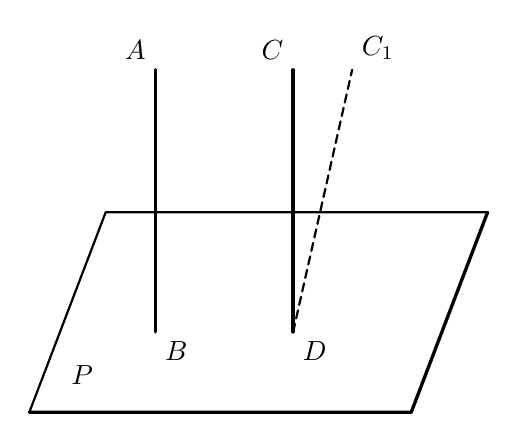
\begin{tikzpicture}[line cap=round,line join=round]
    \coordinate (A) at (-1.25,2.83);
    \coordinate (B) at (-1.25,-0.5);
    \coordinate (C) at (0.5,2.83);
    \coordinate (D) at (0.5,-0.5);
    \coordinate (C1) at (1.25,2.83);
    \draw[thick] (-2.85,-1.52) -- (-1.88,1.02) -- (2.97,1.02);
    \draw[very thick] (-2.85,-1.52) -- (2,-1.52) -- (2.97,1.02);
    \draw[very thick] (A) -- (B) (C) -- (D);
    \draw[thick,densely dashed] (D) -- (C1);
    \node[above left] at (A) {\(A\)};
    \node[below right] at (B) {\(B\)};
    \node[above left] at (C) {\(C\)};
    \node[below right] at (D) {\(D\)};
    \node[above right] at (C1) {\(C_1\)};
    \node at (-2.18,-1.05) {\(P\)};
\end{tikzpicture}

    \caption{Прямые \(AB\) и \(CD\), перпендикулярные к одной плоскости \(P\)}\label{fig:kiselev-stereo-317}
\end{figure}

Предположим противное, то есть что прямые \(AB\) и \(CD\) не параллельны. Проведём тогда через точку \(D\) прямую, параллельную \(AB\). При нашем предположении это будет какая-нибудь прямая \(DC_1\), не совпадающая с \(DC\). Согласно \hyperref[para:plane-perpendicular-to-parallel-lines]{прямой теореме} прямая \(DC_1\) будет перпендикулярна к плоскости \(P\). Тогда у нас будут два перпендикуляра к плоскости \(P\), проходящие через одну и ту же точку, \(DC\) и \(DC_1\). Так как это невозможно, то нельзя допустить, чтобы прямые \(AB\) и \(CD\) были непараллельны.

\kiselevparagraph{para:lines-parallel-to-same-line} \textbf{Теорема. Если две прямые} \(A\) и \(B\) (рис.~\ref{fig:kiselev-stereo-318}) \textbf{параллельны третьей прямой} \(C\)\textbf{, то они параллельны между собой.}

\begin{figure}[htbp]
    \centering
    \renewcommand{\thefigure}{318}
    \captionsetup{name=Рис.,labelsep=period}
    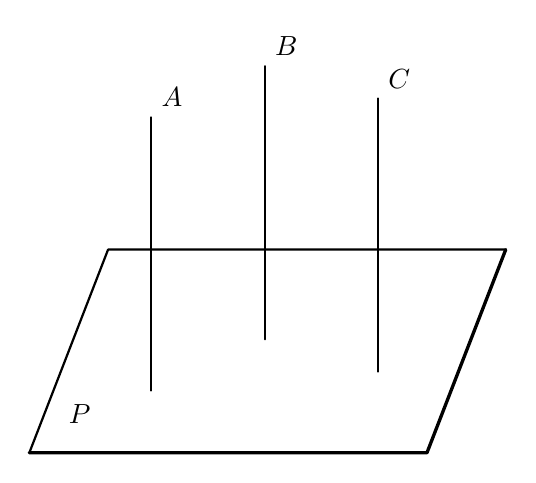
\begin{tikzpicture}[line cap=round,line join=round]
    \draw[thick] (-2.95,-1.62) -- (-1.95,0.96) -- (3.1,0.96);
    \draw[very thick] (-2.95,-1.62) -- (2.1,-1.62) -- (3.1,0.96);
    \draw[thick] (-1.4,-0.83) -- (-1.4,2.64) node[above right] {\(A\)};
    \draw[thick] (0.04,-0.18) -- (0.04,3.29) node[above right] {\(B\)};
    \draw[thick] (1.48,-0.59) -- (1.48,2.88) node[above right] {\(C\)};
    \node at (-2.31,-1.13) {\(P\)};
\end{tikzpicture}

    \caption{Прямые \(A\) и \(B\), параллельные третьей прямой \(C\)}\label{fig:kiselev-stereo-318}
\end{figure}

Проведём плоскость \(P\), перпендикулярную к \(C\). Тогда \(A\) и \(B\) будут перпендикулярны к этой плоскости (\hyperref[para:plane-perpendicular-to-parallel-lines]{см.~§~\ref*{para:plane-perpendicular-to-parallel-lines}}) и, следовательно, \(A\parallel B\) (\hyperref[para:lines-normal-to-same-plane]{см.~§~\ref*{para:lines-normal-to-same-plane}}).

\kiselevparagraph{para:plane-intersection-parallel-to-lines} \textbf{Теорема. Если две прямые} \(A\) и \(B\) (рис.~\ref{fig:kiselev-stereo-319}) \textbf{параллельны и через каждую из них проходит плоскость, то линия пересечения этих плоскостей} (если она существует) \textbf{параллельна первым прямым.}

\begin{figure}[htbp]
    \centering
    \renewcommand{\thefigure}{319}
    \captionsetup{name=Рис.,labelsep=period}
    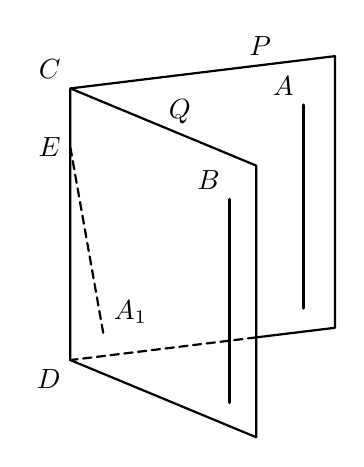
\begin{tikzpicture}[line cap=round,line join=round]
    \coordinate (C) at (-1.91,1.85);
    \coordinate (D) at (-1.91,-1.6);
    \coordinate (E) at (-1.91,1.1);
    \draw[thick] (D) -- (C) -- (1.45,2.26) -- (1.45,-1.19) -- (0.45,-1.312);
    \draw[thick,densely dashed] (0.45,-1.312) -- (D);
    \draw[thick] (C) -- (0.45,0.87) -- (0.45,-2.58) -- (D);
    \draw[very thick] (1.05,1.64) -- (1.05,-0.94);
    \draw[very thick] (0.11,0.44) -- (0.11,-2.14);
    \draw[thick,densely dashed] (E) -- (-1.49,-1.27) node[above right] {\(A_1\)};
    \node[above left] at (C) {\(C\)};
    \node[below left] at (D) {\(D\)};
    \node[left] at (E) {\(E\)};
    \node[above left] at (1.05,1.64) {\(A\)};
    \node[above left] at (0.11,0.44) {\(B\)};
    \node[above] at (0.5,2.14) {\(P\)};
    \node[above] at (-0.52,1.27) {\(Q\)};
\end{tikzpicture}

    \caption{Линия пересечения плоскостей параллельна прямым \(A\) и \(B\)}\label{fig:kiselev-stereo-319}
\end{figure}

% Печатная с. 286.
Пусть через прямую \(A\) проходит плоскость \(P\) и через прямую \(B\) --- плоскость \(Q\), и пусть эти плоскости пересекаются по прямой \(CD\). Требуется доказать, что \(CD\parallel A\) и \(CD\parallel B\). Через какую-нибудь точку \(E\) линии пересечения проведём прямую \(A_1\), параллельную \(A\). Тогда эта прямая должна быть также параллельна \(B\). Так как прямая \(A_1\) параллельна \(A\) и проходит через точку \(E\), то \(A_1\) должна лежать в плоскости, содержащей прямую \(A\) и точку \(E\), то есть в плоскости \(P\). С другой стороны, так как прямая \(A_1\) параллельна \(B\) и проходит через точку \(E\), то \(A_1\) должна лежать в плоскости \(Q\). Если же прямая \(A_1\) лежит одновременно в плоскостях \(P\) и \(Q\), то она должна совпадать с линией пересечения \(CD\). Значит, \(CD\parallel A\) и \(CD\parallel B\).


\section*{Прямая и плоскость, параллельные между собой}
\addcontentsline{toc}{section}{Прямая и плоскость, параллельные между собой}

\kiselevparagraph{para:parallel-line-plane-definition} \textbf{Определение.} Плоскость и прямая, не лежащая в этой плоскости, называются \emph{параллельными}, если они \emph{не пересекаются}, сколько бы их ни продолжали.

Следующие две теоремы выражают \emph{признаки} параллельности прямой с плоскостью.

\kiselevparagraph{para:line-plane-parallel-criteria} \textbf{Теорема 1. Если прямая} \(AB\) (рис.~\ref{fig:kiselev-stereo-320}) \textbf{и плоскость} \(P\) \textbf{перпендикулярны к одной и той же прямой} \(AC\)\textbf{, то они параллельны.}

\begin{figure}[htbp]
    \centering
    \renewcommand{\thefigure}{320}
    \captionsetup{name=Рис.,labelsep=period}
    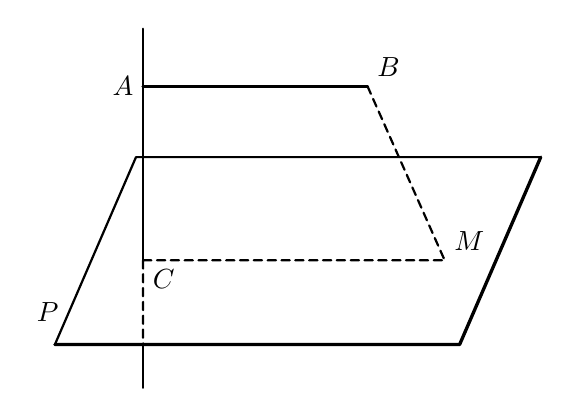
\begin{tikzpicture}[line cap=round,line join=round]
    \coordinate (A) at (-1.83,1.9);
    \coordinate (B) at (1.02,1.9);
    \coordinate (C) at (-1.83,-0.31);
    \coordinate (M) at (2,-0.31);
    \draw[thick] (-2.95,-1.38) -- (-1.92,1.0) -- (3.22,1.0);
    \draw[very thick] (-2.95,-1.38) -- (2.19,-1.38) -- (3.22,1.0);
    \draw[thick] (-1.83,2.63) -- (C) (-1.83,-1.38) -- (-1.83,-1.93);
    \draw[thick,densely dashed] (C) -- (-1.83,-1.38) (C) -- (M) (B) -- (M);
    \draw[very thick] (A) -- (B);
    \node[left] at (A) {\(A\)};
    \node[above right] at (B) {\(B\)};
    \node[below right] at (C) {\(C\)};
    \node[above right] at (M) {\(M\)};
    \node[left] at (-2.78,-0.97) {\(P\)};
\end{tikzpicture}

    \caption{Прямая \(AB\) и плоскость \(P\), перпендикулярные к прямой \(AC\)}\label{fig:kiselev-stereo-320}
\end{figure}

Предположим, что прямая \(AB\) пересекается с плоскостью \(P\) в некоторой точке \(M\). Тогда, соединив прямой эту точку с точкой, в которой плоскость \(P\) пересекается с данной прямой, мы получим два перпендикуляра \(MC\) и \(MA\) на прямую \(AC\) из одной точки \(M\), что невозможно. Значит, \(AB\) не пересекается с \(P\), то есть \(AB\) параллельна \(P\).

% Печатная с. 287.
\textbf{Теорема 2. Если прямая} \(AB\) (рис.~\ref{fig:kiselev-stereo-321}) \textbf{параллельна какой-нибудь прямой} \(CD\)\textbf{, проведённой в плоскости} \(P\)\textbf{, то она параллельна самой плоскости.}

\begin{figure}[htbp]
    \centering
    \renewcommand{\thefigure}{321}
    \captionsetup{name=Рис.,labelsep=period}
    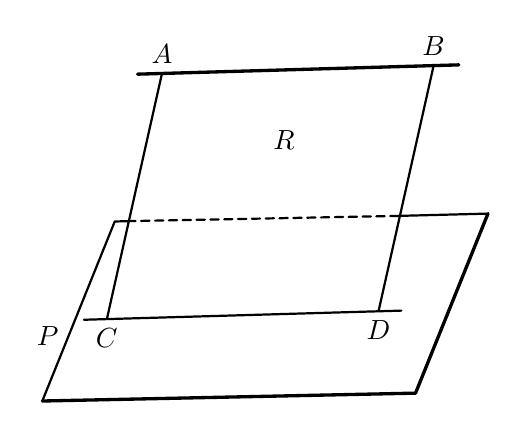
\begin{tikzpicture}[line cap=round,line join=round]
    \coordinate (A) at (-1.28,2.92);
    \coordinate (B) at (2.17,3.02);
    \coordinate (C) at (-1.98,-0.2);
    \coordinate (D) at (1.47,-0.1);
    \draw[thick] (-2.8,-1.24) -- (-1.88,1.04) -- (-1.72,1.044)
        (1.72,1.111) -- (2.86,1.14);
    \draw[thick,densely dashed] (-1.72,1.044) -- (1.72,1.111);
    \draw[very thick] (-2.8,-1.24) -- (1.94,-1.14) -- (2.86,1.14);
    \draw[thick] (A) -- (C) (B) -- (D) (-2.27,-0.208) -- (1.76,-0.092);
    \draw[very thick] (-1.59,2.911) -- (2.49,3.029);
    \node[above] at (A) {\(A\)};
    \node[above] at (B) {\(B\)};
    \node[below] at (C) {\(C\)};
    \node[below] at (D) {\(D\)};
    \node[left] at (-2.47,-0.42) {\(P\)};
    \node at (0.27,2.08) {\(R\)};
\end{tikzpicture}

    \caption{Прямая \(AB\), параллельная прямой \(CD\) в плоскости \(P\)}\label{fig:kiselev-stereo-321}
\end{figure}

Проведём через \(AB\) и \(CD\) плоскость \(R\) и предположим, что прямая \(AB\) где-нибудь пересекается с плоскостью \(P\). Тогда точка пересечения, находясь на прямой \(AB\), должна принадлежать также и плоскости \(R\), в которой лежит \(AB\). В то же время точка пересечения, конечно, должна принадлежать и плоскости \(P\). Значит, точка пересечения, находясь одновременно и в плоскости \(R\), и в плоскости \(P\), должна лежать на прямой \(CD\), по которой пересекаются эти плоскости. Следовательно, прямая \(AB\) пересекается с прямой \(CD\). Но это невозможно, так как, по условию, \(AB\parallel CD\). Значит, нельзя допустить, чтобы прямая \(AB\) пересекалась с плоскостью \(P\), и потому \(AB\parallel P\).

Следующие теоремы выражают некоторые \emph{свойства прямой и плоскости, параллельных между собой}.

\kiselevparagraph{para:parallel-line-plane-section} \textbf{Теорема. Если плоскость} \(R\) (рис.~\ref{fig:kiselev-stereo-321}) \textbf{проходит через прямую} \(AB\)\textbf{, параллельную другой плоскости} \(P\)\textbf{, и пересекает эту плоскость, то линия пересечения} \(CD\) \textbf{параллельна первой прямой} \(AB\)\textbf{.}

Действительно, во-первых, прямая \(CD\) лежит в одной плоскости с \(AB\). Во-вторых, эта прямая не может пересечься с \(AB\), потому что в противном случае прямая \(AB\) пересекалась бы с плоскостью \(P\), что невозможно.

\kiselevparagraph{para:line-parallel-to-two-intersecting-planes} \textbf{Следствие. Если прямая} \(AB\) (рис.~\ref{fig:kiselev-stereo-322}) \textbf{параллельна двум пересекающимся плоскостям} \(P\) и \(Q\)\textbf{, то она параллельна линии их пересечения} \(CD\)\textbf{.}

\begin{figure}[htbp]
    \centering
    \renewcommand{\thefigure}{322}
    \captionsetup{name=Рис.,labelsep=period}
    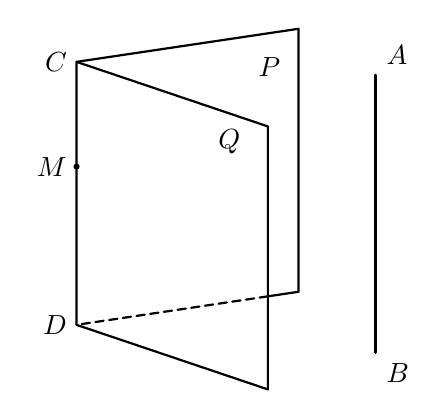
\begin{tikzpicture}[line cap=round,line join=round]
    \coordinate (C) at (-2.1,1.71);
    \coordinate (D) at (-2.1,-1.63);
    \coordinate (M) at (-2.1,0.38);
    \draw[thick] (D) -- (C) -- (0.72,2.13) -- (0.72,-1.21) -- (0.33,-1.268);
    \draw[thick,densely dashed] (0.33,-1.268) -- (D);
    \draw[thick] (C) -- (0.33,0.89) -- (0.33,-2.45) -- (D);
    \draw[very thick] (1.7,1.54) node[above right] {\(A\)}
        -- (1.7,-1.98) node[below right] {\(B\)};
    \fill (M) circle[radius=1.1pt];
    \node[left] at (C) {\(C\)};
    \node[left] at (M) {\(M\)};
    \node[left] at (D) {\(D\)};
    \node at (0.35,1.65) {\(P\)};
    \node at (-0.16,0.69) {\(Q\)};
\end{tikzpicture}

    \caption{Прямая \(AB\), параллельная пересекающимся плоскостям \(P\) и \(Q\)}\label{fig:kiselev-stereo-322}
\end{figure}

Представим плоскость, проходящую через \(AB\) и какую-нибудь точку \(M\) прямой \(CD\). Эта плоскость должна пересечься с \(P\) и \(Q\) по прямым, параллельным \(AB\) и проходящим через \(M\).
% Печатная с. 288.
Но через \(M\) можно провести только одну прямую, параллельную \(AB\). Значит, две линии пересечения этой плоскости с плоскостями \(P\) и \(Q\) должны слиться в одну прямую. Эта прямая, находясь одновременно и в плоскости \(P\), и в плоскости \(Q\), должна совпадать с прямой \(CD\), по которой плоскости \(P\) и \(Q\) пересекаются. Значит, \(CD\parallel AB\).

\kiselevparagraph{para:distance-from-parallel-line-to-plane} \textbf{Теорема. Все точки прямой} \(AB\) (рис.~\ref{fig:kiselev-stereo-323})\textbf{, параллельной плоскости} \(P\)\textbf{, одинаково удалены от этой плоскости.}

\begin{figure}[htbp]
    \centering
    \renewcommand{\thefigure}{323}
    \captionsetup{name=Рис.,labelsep=period}
    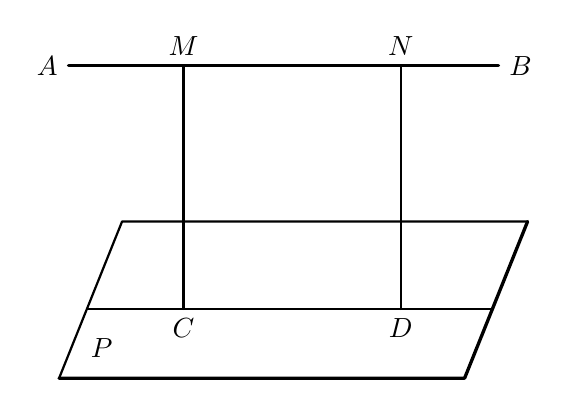
\begin{tikzpicture}[line cap=round,line join=round]
    \coordinate (M) at (-1.27,2.85);
    \coordinate (N) at (1.49,2.85);
    \coordinate (C) at (-1.27,-0.24);
    \coordinate (D) at (1.49,-0.24);
    \draw[thick] (-2.85,-1.12) -- (-2.05,0.87) -- (3.1,0.87);
    \draw[very thick] (-2.85,-1.12) -- (2.3,-1.12) -- (3.1,0.87);
    \draw[thick] (-2.495,-0.24) -- (2.655,-0.24) (M) -- (C) (N) -- (D);
    \draw[very thick] (-2.73,2.85) node[left] {\(A\)} -- (2.73,2.85) node[right] {\(B\)};
    \node[above] at (M) {\(M\)};
    \node[above] at (N) {\(N\)};
    \node[below] at (C) {\(C\)};
    \node[below] at (D) {\(D\)};
    \node at (-2.31,-0.74) {\(P\)};
\end{tikzpicture}

    \caption{Точки прямой \(AB\) одинаково удалены от плоскости \(P\)}\label{fig:kiselev-stereo-323}
\end{figure}

Из каких-нибудь точек \(M\) и \(N\) прямой \(AB\) опустим на \(P\) перпендикуляры \(MC\) и \(ND\). Так как эти перпендикуляры параллельны (\hyperref[para:lines-normal-to-same-plane]{см.~§~\ref*{para:lines-normal-to-same-plane}}), то через них можно провести плоскость. Эта плоскость пересекается с \(P\) по прямой \(CD\), параллельной \(AB\) (\hyperref[para:parallel-line-plane-section]{см.~§~\ref*{para:parallel-line-plane-section}}). Поэтому фигура \(MNDC\) --- параллелограмм и, следовательно, \(MC=ND\). Но длину перпендикуляра, опущенного из точки на плоскость, принимают за меру расстояния этой точки от плоскости. Значит, любые точки \(M\) и \(N\) прямой \(AB\) одинаково удалены от плоскости \(P\).


\section*{Параллельные плоскости}
\addcontentsline{toc}{section}{Параллельные плоскости}

\kiselevparagraph{para:parallel-planes-definition} \textbf{Определение.} Две плоскости называются \emph{параллельными}, если они \emph{не пересекаются, сколько бы их ни продолжали}.

Следующие две теоремы выражают \emph{признаки} параллельности двух плоскостей.

\kiselevparagraph{para:parallel-planes-criteria} \textbf{Теорема 1. Если две плоскости} \(P\) и \(Q\) (рис.~\ref{fig:kiselev-stereo-324}) \textbf{перпендикулярны к одной и той же прямой} \(AB\)\textbf{, то они параллельны.}

\begin{figure}[htbp]
    \centering
    \renewcommand{\thefigure}{324}
    \captionsetup{name=Рис.,labelsep=period}
    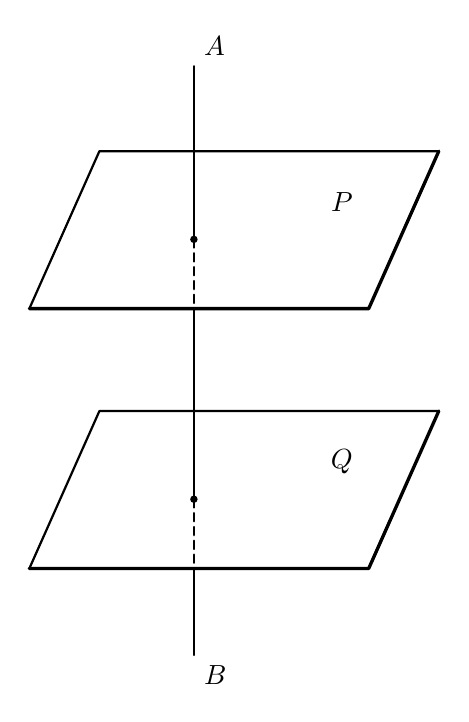
\begin{tikzpicture}[line cap=round,line join=round]
    \foreach \height/\plane in {0.6/P,-2.7/Q}{
        \begin{scope}[yshift=\height cm]
            \draw[thick] (-2.62,0) -- (-1.73,2) -- (2.58,2);
            \draw[very thick] (-2.62,0) -- (1.69,0) -- (2.58,2);
            \node at (1.35,1.36) {\(\plane\)};
        \end{scope}
    }
    \draw[thick] (-0.53,3.68) node[above right] {\(A\)} -- (-0.53,1.48)
        (-0.53,0.6) -- (-0.53,-1.82) (-0.53,-2.7) -- (-0.53,-3.8) node[below right] {\(B\)};
    \draw[thick,densely dashed] (-0.53,1.48) -- (-0.53,0.6)
        (-0.53,-1.82) -- (-0.53,-2.7);
    \fill (-0.53,1.48) circle[radius=1.35pt];
    \fill (-0.53,-1.82) circle[radius=1.35pt];
\end{tikzpicture}

    \caption{Плоскости \(P\) и \(Q\), перпендикулярные к одной прямой \(AB\)}\label{fig:kiselev-stereo-324}
\end{figure}

Действительно, если бы плоскости \(P\) и \(Q\) пересекались, то через любую точку их пересечения проходили бы две плоскости \(P\) и \(Q\), перпендикулярные к прямой \(AB\), что невозможно.

% Печатная с. 289.
\phantomsection\label{thm:parallel-planes-two-lines}
\textbf{Теорема 2. Если две пересекающиеся прямые} \(AB\) и \(AC\) (рис.~\ref{fig:kiselev-stereo-325}) \textbf{одной плоскости} \(P\) \textbf{соответственно параллельны двум прямым} \(A_1B_1\) и \(A_1C_1\) \textbf{другой плоскости} \(Q\)\textbf{, то эти плоскости параллельны.}

\begin{figure}[htbp]
    \centering
    \renewcommand{\thefigure}{325}
    \captionsetup{name=Рис.,labelsep=period}
    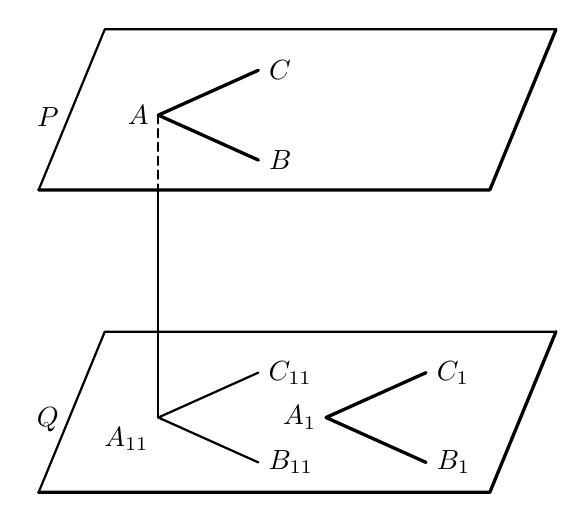
\begin{tikzpicture}[line cap=round,line join=round]
    \coordinate (A) at (-1.75,1.69);
    \coordinate (A11) at (-1.75,-2.15);
    \coordinate (A1) at (0.38,-2.15);
    \foreach \height/\plane in {0.74/P,-3.1/Q}{
        \begin{scope}[yshift=\height cm]
            \draw[thick] (-3.27,0) -- (-2.43,2.04) -- (3.3,2.04);
            \draw[very thick] (-3.27,0) -- (2.46,0) -- (3.3,2.04);
            \node[left] at (-2.89,0.92) {\(\plane\)};
        \end{scope}
    }
    \draw[thick,densely dashed] (A) -- (-1.75,0.74);
    \draw[thick] (-1.75,0.74) -- (A11);
    \draw[very thick] (-0.48,2.26) node[right] {\(C\)} -- (A) -- (-0.48,1.12) node[right] {\(B\)};
    \draw[thick] (-0.48,-1.58) node[right] {\(C_{11}\)} -- (A11)
        -- (-0.48,-2.72) node[right] {\(B_{11}\)};
    \draw[very thick] (1.65,-1.58) node[right] {\(C_1\)} -- (A1)
        -- (1.65,-2.72) node[right] {\(B_1\)};
    \node[left] at (A) {\(A\)};
    \node[below left] at (A11) {\(A_{11}\)};
    \node[left] at (A1) {\(A_1\)};
\end{tikzpicture}

    \caption{Соответственно параллельные прямые в плоскостях \(P\) и \(Q\)}\label{fig:kiselev-stereo-325}
\end{figure}

Из точки \(A\) опустим на плоскость \(Q\) перпендикуляр \(AA_{11}\) и проведём прямые \(A_{11}B_{11}\) и \(A_{11}C_{11}\), соответственно параллельные прямым \(A_1B_1\) и \(A_1C_1\). Эти прямые также параллельны прямым \(AB\) и \(AC\) (\hyperref[para:lines-parallel-to-same-line]{см.~§~\ref*{para:lines-parallel-to-same-line}}). Так как \(AA_{11}\perp A_{11}B_{11}\) и \(AB\parallel A_{11}B_{11}\), то \(AA_{11}\perp AB\). Так же доказывается, что \(AA_{11}\perp AC\). Следовательно, прямая \(AA_{11}\) перпендикулярна к плоскости \(P\) (\hyperref[para:perpendicular-plane-criterion]{см.~§~\ref*{para:perpendicular-plane-criterion}}). Таким образом, плоскости \(P\) и \(Q\) перпендикулярны к одной и той же прямой \(AA_{11}\) и потому параллельны.

Следующие теоремы выражают некоторые \emph{свойства параллельных плоскостей}.

\kiselevparagraph{para:sections-of-parallel-planes} \textbf{Теорема. Если две параллельные плоскости} \(P\) и \(Q\) (рис.~\ref{fig:kiselev-stereo-326}) \textbf{пересекаются третьей плоскостью} \(R\)\textbf{, то линии пересечения} \(AC\) и \(BD\) \textbf{параллельны.}

\begin{figure}[htbp]
    \centering
    \renewcommand{\thefigure}{326}
    \captionsetup{name=Рис.,labelsep=period}
    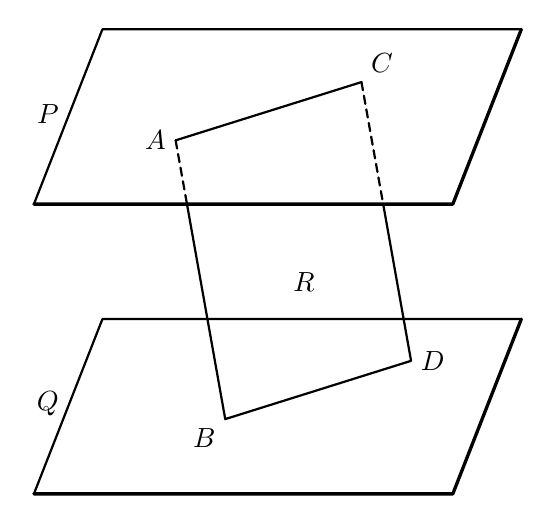
\begin{tikzpicture}[line cap=round,line join=round]
    \coordinate (A) at (-1.32,1.45);
    \coordinate (C) at (1.04,2.19);
    \coordinate (B) at (-0.69,-2.09);
    \coordinate (D) at (1.67,-1.35);
    \path (A) -- (B) coordinate[pos=0.2288] (frontA);
    \path (C) -- (D) coordinate[pos=0.4379] (frontC);
    \foreach \height/\plane in {0.64/P,-3.04/Q}{
        \begin{scope}[yshift=\height cm]
            \draw[thick] (-3.12,0) -- (-2.25,2.22) -- (3.07,2.22);
            \draw[very thick] (-3.12,0) -- (2.2,0) -- (3.07,2.22);
            \node[left] at (-2.68,1.14) {\(\plane\)};
        \end{scope}
    }
    \draw[thick] (A) -- (C) (frontA) -- (B) -- (D) -- (frontC);
    \draw[thick,densely dashed] (A) -- (frontA) (C) -- (frontC);
    \node[left] at (A) {\(A\)};
    \node[above right] at (C) {\(C\)};
    \node[below left] at (B) {\(B\)};
    \node[right] at (D) {\(D\)};
    \node at (0.31,-0.35) {\(R\)};
\end{tikzpicture}

    \caption{Линии пересечения параллельных плоскостей \(P\) и \(Q\) с плоскостью \(R\)}\label{fig:kiselev-stereo-326}
\end{figure}

Действительно, во-первых, прямые \(AC\) и \(BD\) находятся в одной плоскости \(R\). Во-вторых, они не могут пересечься, так как в противном случае пересекались бы плоскости \(P\) и \(Q\), что противоречит условию.

\kiselevparagraph{para:transversals-of-parallel-planes} \textbf{Теоремы.}

\begin{enumerate}[label=\arabic*),ref=\arabic*]
    \item \textbf{Если прямая пересекает одну из параллельных плоскостей, то она пересекает и другую.}
    \item \textbf{Если плоскость пересекает одну из параллельных плоскостей, то она пересекает и другую.}
\end{enumerate}

\begin{figure}[htbp]
    \centering
    \renewcommand{\thefigure}{327}
    \captionsetup{name=Рис.,labelsep=period}
    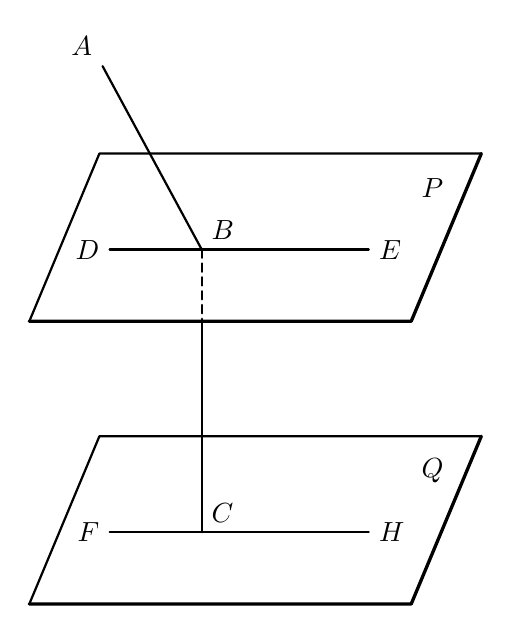
\begin{tikzpicture}[line cap=round,line join=round]
    \coordinate (B) at (-0.72,1.47);
    \coordinate (C) at (-0.72,-2.12);
    \foreach \height/\plane in {0.56/P,-3.03/Q}{
        \begin{scope}[yshift=\height cm]
            \draw[thick] (-2.91,0) -- (-2.02,2.13) -- (2.83,2.13);
            \draw[very thick] (-2.91,0) -- (1.94,0) -- (2.83,2.13);
            \node at (2.21,1.69) {\(\plane\)};
        \end{scope}
    }
    \draw[thick] (-1.98,3.8) node[above left] {\(A\)} -- (B);
    \draw[thick,densely dashed] (B) -- (-0.72,0.56);
    \draw[thick] (-0.72,0.56) -- (C);
    \draw[thick] (-1.89,1.47) node[left] {\(D\)} -- (1.4,1.47) node[right] {\(E\)};
    \draw[thick] (-1.89,-2.12) node[left] {\(F\)} -- (1.4,-2.12) node[right] {\(H\)};
    \node[above right] at (B) {\(B\)};
    \node[above right] at (C) {\(C\)};
\end{tikzpicture}

    \caption{Пересечение параллельных плоскостей \(P\) и \(Q\)}\label{fig:kiselev-stereo-327}
\end{figure}

\begin{enumerate}[label=\arabic*),ref=\arabic*]
    \item\label{item:line-intersects-both-parallel-planes} Пусть прямая \(AB\) (рис.~\ref{fig:kiselev-stereo-327}) пересекает в точке \(B\) плоскость \(P\), параллельную \(Q\). Соединим прямой точку \(B\) с какой-нибудь точкой плоскости \(Q\)
    % Печатная с. 290.
    и через \(AB\) и \(BC\) проведём плоскость, не указанную на рисунке. Эта плоскость, содержащая точки \(B\) и \(C\), пересекается с \(P\) и \(Q\) по некоторым прямым \(DE\) и \(FH\), которые параллельны (\hyperref[para:sections-of-parallel-planes]{см.~§~\ref*{para:sections-of-parallel-planes}}). Прямая \(AB\) лежит в одной плоскости с \(DE\) и \(FH\) и пересекает одну из этих параллельных. Следовательно, как мы знаем из планиметрии (\kiselevPlanimetryPage{71}{см.~§~80, пункт~1}), она пересечёт и другую, а значит, пересечёт и плоскость \(Q\).
    \item Пусть какая-нибудь плоскость пересекает плоскость \(P\) (рис.~\ref{fig:kiselev-stereo-327}), параллельную \(Q\). Тогда на ней можно взять прямую \(AB\), которая тоже пересекает плоскость \(P\). \hyperref[item:line-intersects-both-parallel-planes]{По доказанному} эта прямая пересекает и плоскость \(Q\). Значит, с этой плоскостью пересечётся и та плоскость, в которой взята \(AB\).
\end{enumerate}

\kiselevparagraph{para:line-normal-to-parallel-planes} \textbf{Теорема. Если прямая} \(AB\) (рис.~\ref{fig:kiselev-stereo-328}) \textbf{перпендикулярна к одной из параллельных плоскостей} \(P\)\textbf{, то она перпендикулярна и к~другой}~\(Q\)\textbf{.}

\begin{figure}[htbp]
    \centering
    \renewcommand{\thefigure}{328}
    \captionsetup{name=Рис.,labelsep=period}
    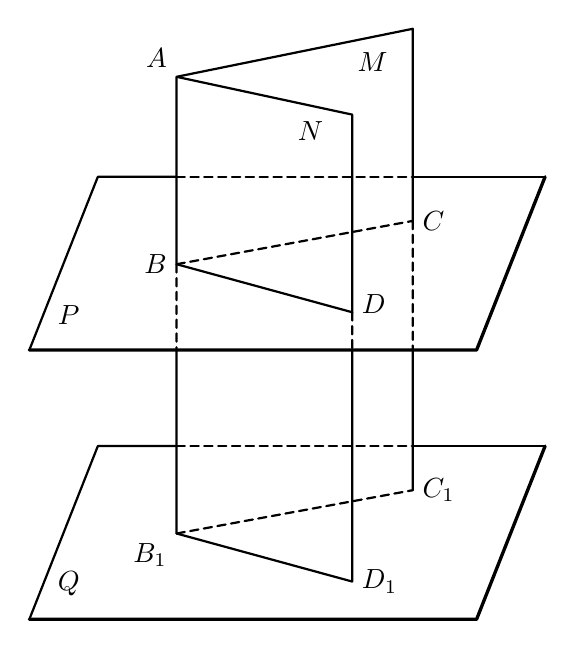
\begin{tikzpicture}[line cap=round,line join=round]
    \coordinate (A) at (-1.47,3.53);
    \coordinate (B) at (-1.47,1.15);
    \coordinate (B1) at (-1.47,-2.27);
    \coordinate (C) at (1.53,1.7);
    \coordinate (C1) at (1.53,-1.72);
    \coordinate (D) at (0.76,0.54);
    \coordinate (D1) at (0.76,-2.88);
    \foreach \height/\plane in {0.06/P,-3.36/Q}{
        \begin{scope}[yshift=\height cm]
            \draw[thick] (-3.34,0) -- (-2.47,2.2) -- (-1.47,2.2);
            \draw[thick,densely dashed] (-1.47,2.2) -- (1.53,2.2);
            \draw[thick] (1.53,2.2) -- (3.21,2.2);
            \draw[very thick] (-3.34,0) -- (2.34,0) -- (3.21,2.2);
            \node at (-2.84,0.45) {\(\plane\)};
        \end{scope}
    }
    \draw[thick] (A) -- (1.53,4.14) -- (C)
        (A) -- (0.76,3.05) -- (D) -- (B) -- (A);
    \draw[thick,densely dashed] (B) -- (C)
        (B) -- (-1.47,0.06) (C) -- (1.53,0.06) (D) -- (0.76,0.06)
        (B1) -- (C1);
    \draw[thick] (-1.47,0.06) -- (B1) -- (D1) -- (0.76,0.06)
        (1.53,0.06) -- (C1);
    \node[above left] at (A) {\(A\)};
    \node[left] at (B) {\(B\)};
    \node[below left] at (B1) {\(B_1\)};
    \node[right] at (C) {\(C\)};
    \node[right] at (C1) {\(C_1\)};
    \node[right,yshift=3pt] at (D) {\(D\)};
    \node[right] at (D1) {\(D_1\)};
    \node at (1.02,3.72) {\(M\)};
    \node at (0.23,2.84) {\(N\)};
\end{tikzpicture}

    \caption{Прямая \(AB\), перпендикулярная к параллельным плоскостям \(P\) и \(Q\)}\label{fig:kiselev-stereo-328}
\end{figure}

Прямая \(AB\), пересекая одну из параллельных плоскостей, пересечёт и другую в некоторой точке \(B_1\). Проведём через \(AB\) какие-нибудь две плоскости \(M\) и \(N\), которые пересекутся с \(P\) и \(Q\) по параллельным прямым (\hyperref[para:sections-of-parallel-planes]{см.~§~\ref*{para:sections-of-parallel-planes}}): одна по \(BC\) и \(B_1C_1\), другая по \(BD\) и \(B_1D_1\). Согласно условию, прямая \(AB\) перпендикулярна к \(BC\) и \(BD\). Следовательно, она также перпендикулярна к \(B_1C_1\) и \(B_1D_1\), а потому перпендикулярна и к плоскости \(Q\).

\kiselevparagraph{para:unique-parallel-plane-through-point} \textbf{Теорема. Через любую точку} \(B\) (рис.~\ref{fig:kiselev-stereo-328}) \textbf{пространства можно провести плоскость} \(P\)\textbf{, параллельную данной плоскости} \(Q\)\textbf{, и притом только одну.}

Всегда можно из точки \(B\) опустить на плоскость \(Q\) перпендикуляр \(BB_1\) и затем через точку \(B\) провести плоскость \(P\), перпендикулярную к \(BB_1\). Эта плоскость будет параллельна \(Q\) (\hyperref[para:parallel-planes-criteria]{см.~§~\ref*{para:parallel-planes-criteria}, теорема~1}).

% Печатная с. 291.
Другой плоскости, параллельной \(Q\), через точку \(B\) провести нельзя, так как, если бы это было возможно, то через точку \(B\) проходили бы две плоскости, перпендикулярные к \(BB_1\) (\hyperref[para:line-normal-to-parallel-planes]{см.~§~\ref*{para:line-normal-to-parallel-planes}}), что невозможно.

\kiselevparagraph{para:equal-segments-between-parallel-planes} \textbf{Теорема. Отрезки параллельных прямых} \(AC\) и \(BD\) (рис.~\ref{fig:kiselev-stereo-329})\textbf{, заключённые между параллельными плоскостями} \(P\) и \(Q\)\textbf{, равны.}

\begin{figure}[htbp]
    \centering
    \renewcommand{\thefigure}{329}
    \captionsetup{name=Рис.,labelsep=period}
    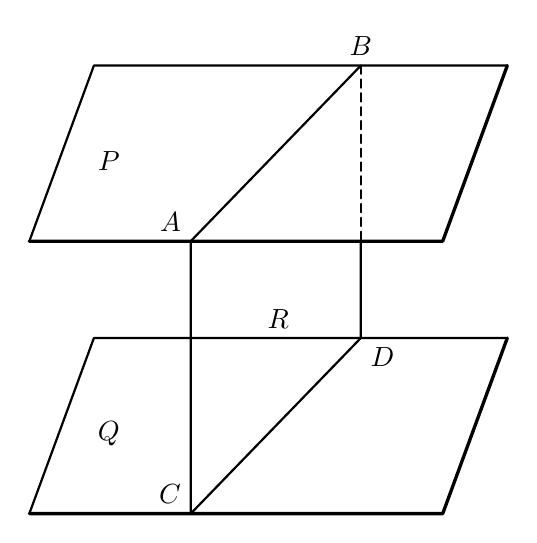
\begin{tikzpicture}[line cap=round,line join=round]
    \coordinate (A) at (-1.0,0.57);
    \coordinate (B) at (1.16,2.8);
    \coordinate (C) at (-1.0,-2.89);
    \coordinate (D) at (1.16,-0.66);
    \foreach \height/\plane in {0.57/P,-2.89/Q}{
        \begin{scope}[yshift=\height cm]
            \draw[thick] (-3.05,0) -- (-2.23,2.23) -- (3.02,2.23);
            \draw[very thick] (-3.05,0) -- (2.2,0) -- (3.02,2.23);
            \node at (-2.04,1.02) {\(\plane\)};
        \end{scope}
    }
    \draw[thick] (A) -- (B) (C) -- (D) (A) -- (C) (1.16,0.57) -- (D);
    \draw[thick,densely dashed] (B) -- (1.16,0.57);
    \node[above left] at (A) {\(A\)};
    \node[above] at (B) {\(B\)};
    \node[above left] at (C) {\(C\)};
    \node[below right] at (D) {\(D\)};
    \node at (0.11,-0.42) {\(R\)};
\end{tikzpicture}

    \caption{Равные отрезки \(AC\) и \(BD\) между параллельными плоскостями}\label{fig:kiselev-stereo-329}
\end{figure}

Через параллельные прямые \(AC\) и \(BD\) проведём плоскость \(R\). Она пересечёт \(P\) и \(Q\) по параллельным прямым \(AB\) и \(CD\). Следовательно, фигура \(ABCD\)\footnote{В издании 1914 года указан порядок \(ABCD\). На рис.~\ref{fig:kiselev-stereo-329} при обходе по сторонам вершины идут в порядке \(A,B,D,C\).} будет параллелограммом, и потому \(AC=BD\).

\kiselevparagraph{para:parallel-planes-equidistant} \textbf{Следствие. Параллельные плоскости везде одинаково удалены одна от другой}, потому что, если параллельные прямые \(AC\) и \(BD\) (рис.~\ref{fig:kiselev-stereo-329}) перпендикулярны к \(P\), то они также будут перпендикулярны к \(Q\) и в то же время равны.

\kiselevparagraph{para:angles-with-parallel-sides} \textbf{Теорема. Два угла} \(BAC\) и \(B_1A_1C_1\) (рис.~\ref{fig:kiselev-stereo-330}) \textbf{с соответственно параллельными и одинаково направленными сторонами равны и лежат в параллельных плоскостях} \(P\) и \(Q\)\textbf{.}

\begin{figure}[htbp]
    \centering
    \renewcommand{\thefigure}{330}
    \captionsetup{name=Рис.,labelsep=period}
    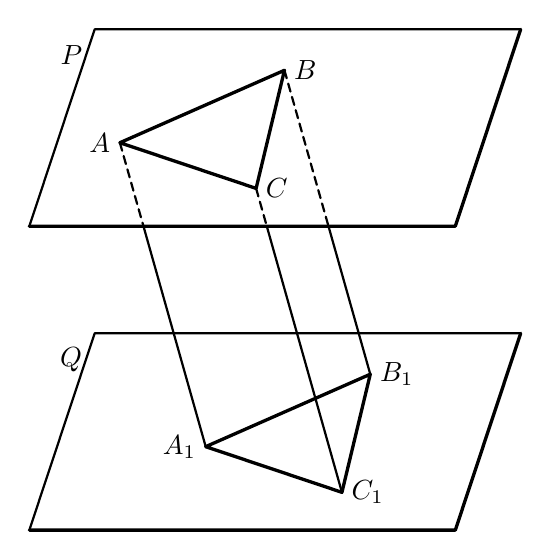
\begin{tikzpicture}[line cap=round,line join=round]
    \coordinate (A) at (-1.93,1.58);
    \coordinate (B) at (0.16,2.5);
    \coordinate (C) at (-0.2,1.0);
    \coordinate (A1) at (-0.84,-2.28);
    \coordinate (B1) at (1.25,-1.36);
    \coordinate (C1) at (0.89,-2.86);
    \foreach \height/\plane in {0.52/P,-3.34/Q}{
        \begin{scope}[yshift=\height cm]
            \draw[thick] (-3.08,0) -- (-2.25,2.5) -- (3.16,2.5);
            \draw[very thick] (-3.08,0) -- (2.33,0) -- (3.16,2.5);
            \node[left,xshift=-3pt] at (-2.18,2.17) {\(\plane\)};
        \end{scope}
    }
    \path (A) -- (A1) coordinate[pos=0.2746] (frontA);
    \path (B) -- (B1) coordinate[pos=0.5130] (frontB);
    \path (C) -- (C1) coordinate[pos=0.1244] (frontC);
    \draw[thick,densely dashed] (A) -- (frontA) (B) -- (frontB) (C) -- (frontC);
    \draw[thick] (frontA) -- (A1) (frontB) -- (B1) (frontC) -- (C1);
    \draw[very thick] (A) -- (B) -- (C) -- cycle (A1) -- (B1) -- (C1) -- cycle;
    \node[left] at (A) {\(A\)};
    \node[right] at (B) {\(B\)};
    \node[right] at (C) {\(C\)};
    \node[left] at (A1) {\(A_1\)};
    \node[right] at (B1) {\(B_1\)};
    \node[right] at (C1) {\(C_1\)};
\end{tikzpicture}

    \caption{Углы \(BAC\) и \(B_1A_1C_1\) с соответственно параллельными сторонами}\label{fig:kiselev-stereo-330}
\end{figure}

То, что плоскости \(P\) и \(Q\) параллельны, было доказано прежде (\hyperref[thm:parallel-planes-two-lines]{см.~§~\ref*{para:parallel-planes-criteria}, теорема~2}). Остаётся доказать, что углы \(A\) и \(A_1\) равны.

Отложим \(AB=A_1B_1\), \(AC=A_1C_1\) и проведём \(AA_1\), \(BB_1\), \(CC_1\), \(BC\) и \(B_1C_1\). Так как отрезки \(AB\) и \(A_1B_1\) равны и параллельны, то фигура \(ABB_1A_1\) является параллелограммом (\kiselevPlanimetryPage{85}{см.~Планиметрия, §~99, пункт~2}). Поэтому отрезки \(AA_1\) и \(BB_1\) равны и параллельны. По той же причине равны и параллельны отрезки \(AA_1\) и \(CC_1\). Следовательно, \(BB_1\parallel CC_1\) и \(BB_1=CC_1\). Поэтому \(BC=B_1C_1\) и \(\triangle ABC=\triangle A_1B_1C_1\) (по трём сторонам). Значит, \(\angle A=\angle A_1\).

% Печатная с. 292.
\kiselevparagraph{para:parallel-planes-proportional-segments} \textbf{Теорема. Если две прямые} \(AB\) и \(CD\) (рис.~\ref{fig:kiselev-stereo-331}) \textbf{пересекаются рядом параллельных плоскостей} \(P,Q,R,\ldots\)\textbf{, то эти плоскости делят их на пропорциональные части.}

\begin{figure}[htbp]
    \centering
    \renewcommand{\thefigure}{331}
    \captionsetup{name=Рис.,labelsep=period}
    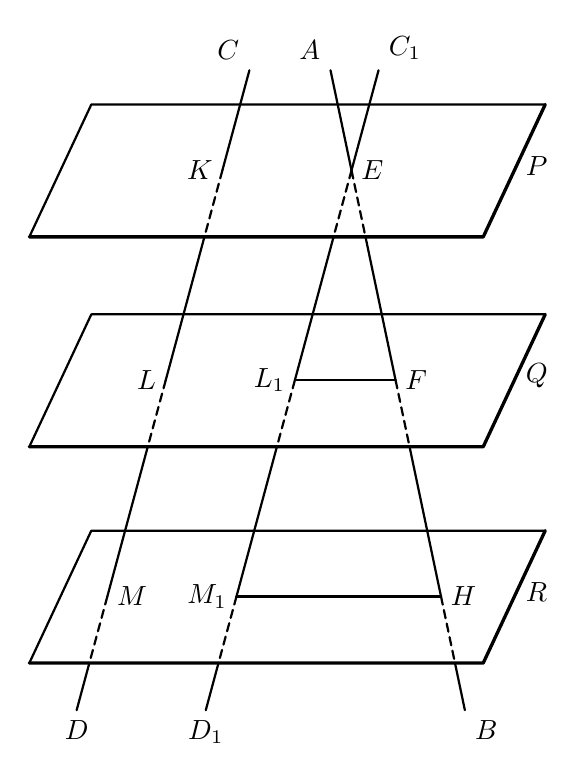
\begin{tikzpicture}[line cap=round,line join=round,scale=0.82]
    \coordinate (E) at (0.05,4.2);
    \coordinate (F) at (0.7325,0.95);
    \coordinate (H) at (1.436,-2.4);
    \coordinate (K) at (-1.95,4.2);
    \coordinate (L) at (-2.8275,0.95);
    \coordinate (M) at (-3.732,-2.4);
    \coordinate (L1) at (-0.8275,0.95);
    \coordinate (M1) at (-1.732,-2.4);
    \foreach \height/\plane in {3.17/P,-0.08/Q,-3.43/R}{
        \begin{scope}[yshift=\height cm]
            \draw[thick] (-4.94,0) -- (-3.98,2.05) -- (3.05,2.05);
            \draw[very thick] (-4.94,0) -- (2.09,0) -- (3.05,2.05);
            \node[right] at (2.6,1.1) {\(\plane\)};
        \end{scope}
    }
    \path (E) -- (F) coordinate[pos=0.3169] (frontE);
    \path (F) -- (H) coordinate[pos=0.3075] (frontF);
    \path (H) -- (1.8056,-4.16) coordinate[pos=0.5852] (frontH);
    \path (K) -- (L) coordinate[pos=0.3169] (frontK);
    \path (L) -- (M) coordinate[pos=0.3075] (frontL);
    \path (M) -- (-4.2072,-4.16) coordinate[pos=0.5852] (frontM);
    \path (E) -- (L1) coordinate[pos=0.3169] (frontE1);
    \path (L1) -- (M1) coordinate[pos=0.3075] (frontL1);
    \path (M1) -- (-2.2072,-4.16) coordinate[pos=0.5852] (frontM1);

    \draw[thick,densely dashed] (E) -- (frontE) (F) -- (frontF) (H) -- (frontH)
        (K) -- (frontK) (L) -- (frontL) (M) -- (frontM)
        (E) -- (frontE1) (L1) -- (frontL1) (M1) -- (frontM1);
    \draw[thick] (-0.2755,5.75) node[above left] {\(A\)} -- (E)
        (frontE) -- (F) (frontF) -- (H)
        (frontH) -- (1.8056,-4.16) node[below right] {\(B\)};
    \draw[thick] (-1.5315,5.75) node[above left] {\(C\)} -- (K)
        (frontK) -- (L) (frontL) -- (M)
        (frontM) -- (-4.2072,-4.16) node[below] {\(D\)};
    \draw[thick] (0.4685,5.75) node[above right] {\(C_1\)} -- (E)
        (frontE1) -- (L1) (frontL1) -- (M1)
        (frontM1) -- (-2.2072,-4.16) node[below] {\(D_1\)};
    \draw[thick] (L1) -- (F) (M1) -- (H);
    \node[right] at (E) {\(E\)};
    \node[right] at (F) {\(F\)};
    \node[right] at (H) {\(H\)};
    \node[left] at (K) {\(K\)};
    \node[left] at (L) {\(L\)};
    \node[right] at (M) {\(M\)};
    \node[left] at (L1) {\(L_1\)};
    \node[left] at (M1) {\(M_1\)};
\end{tikzpicture}

    \caption{Пропорциональные отрезки между параллельными плоскостями}\label{fig:kiselev-stereo-331}
\end{figure}

Пусть \(E,F,H,\ldots\) --- точки пересечения прямой \(AB\) с плоскостями \(P,Q,R,\ldots\), а \(K,L,M,\ldots\) --- точки пересечения другой прямой \(CD\) с теми же плоскостями. Требуется доказать, что части \(EF,FH,\ldots\) одной прямой пропорциональны частям \(KL,LM,\ldots\) другой прямой, то есть
\[
    \frac{EF}{KL}=\frac{FH}{LM}=\cdots.
\]

Проведём через точку \(E\) прямую \(C_1D_1\), параллельную \(CD\), и представим плоскость, проходящую через две пересекающиеся прямые \(AB\) и \(C_1D_1\). Прямые \(L_1F,M_1H,\ldots\), по которым эта плоскость пересекается с данными плоскостями, должны быть параллельны между собой (\hyperref[para:sections-of-parallel-planes]{см.~§~\ref*{para:sections-of-parallel-planes}}). Поэтому (\kiselevPlanimetryPage{171}{см.~Планиметрия, §~219})\footnote{В первом знаменателе этой формулы в издании 1914 года напечатано \(E_1L_1\). На рис.~\ref{fig:kiselev-stereo-331} отмечена точка \(E\), а далее в доказательстве используется отрезок \(EL_1\).}
\[
    \frac{EF}{E_1L_1}=\frac{FH}{L_1M_1}=\cdots.
\]

Но \(EL_1=KL\), \(L_1M_1=LM,\ldots\) (\hyperref[para:equal-segments-between-parallel-planes]{см.~§~\ref*{para:equal-segments-between-parallel-planes}}). Подставив в полученный ряд равных отношений отрезки \(KL,LM,\ldots\) вместо \(EL_1,L_1M_1,\ldots\), получим то, что требовалось доказать.

\clearpage
\endgroup
